\section{Date: 2026-10-29}
\noindent \textbf{Series ID: COVEMP} 

\noindent This series is titled Covered Employment and has a frequency of Weekly, Ending Saturday. The units are Number and the seasonal adjustment is Not Seasonally Adjusted.The observation start date is 1971-01-02 and the observation end date is 2026-10-10.The popularity of this series is 16. \\ 

\noindent \textbf{Series ID: PONHPI00106M226N} 

\noindent This series is titled Purchase Only House Price Index for the East North Central Census Division and has a frequency of Monthly. The units are Index Jan 1991=100 and the seasonal adjustment is Not Seasonally Adjusted.The observation start date is 1991-01-01 and the observation end date is 2026-08-01.The popularity of this series is 1. \\ 

\subsection{Raw Regression}
\noindent Regresses the two series against each other directly. A significant result here can come just as easily from both series sharing a long-run trend as from any real relationship.

\begin{center}
\begin{tabular}{lclc}
\toprule
\textbf{Dep. Variable:}      & value\_fred\_PONHPI00106M226N & \textbf{  R-squared:         } &     0.787   \\
\textbf{Model:}              &              OLS              & \textbf{  Adj. R-squared:    } &     0.784   \\
\textbf{Method:}             &         Least Squares         & \textbf{  F-statistic:       } &     218.3   \\
\textbf{Date:}               &        Thu, 29 Oct 2026       & \textbf{  Prob (F-statistic):} &  1.72e-21   \\
\textbf{Time:}               &            17:40:13           & \textbf{  Log-Likelihood:    } &   -300.50   \\
\textbf{No. Observations:}   &                 61            & \textbf{  AIC:               } &     605.0   \\
\textbf{Df Residuals:}       &                 59            & \textbf{  BIC:               } &     609.2   \\
\textbf{Df Model:}           &                  1            & \textbf{                     } &             \\
\textbf{Covariance Type:}    &           nonrobust           & \textbf{                     } &             \\
\bottomrule
\end{tabular}
\begin{tabular}{lcccccc}
                             & \textbf{coef} & \textbf{std err} & \textbf{t} & \textbf{P$> |$t$|$} & \textbf{[0.025} & \textbf{0.975]}  \\
\midrule
\textbf{const}               &    -444.7300  &       43.423     &   -10.242  &         0.000        &     -531.619    &     -357.841     \\
\textbf{value\_fred\_COVEMP} &    4.924e-06  &     3.33e-07     &    14.776  &         0.000        &     4.26e-06    &     5.59e-06     \\
\bottomrule
\end{tabular}
\begin{tabular}{lclc}
\textbf{Omnibus:}       &  6.707 & \textbf{  Durbin-Watson:     } &    0.108  \\
\textbf{Prob(Omnibus):} &  0.035 & \textbf{  Jarque-Bera (JB):  } &    4.815  \\
\textbf{Skew:}          &  0.551 & \textbf{  Prob(JB):          } &   0.0900  \\
\textbf{Kurtosis:}      &  2.174 & \textbf{  Cond. No.          } & 1.30e+09  \\
\bottomrule
\end{tabular}
%\caption{OLS Regression Results}
\end{center}

Notes: \newline
 [1] Standard Errors assume that the covariance matrix of the errors is correctly specified. \newline
 [2] The condition number is large, 1.3e+09. This might indicate that there are \newline
 strong multicollinearity or other numerical problems.

\begin{figure}
\centering
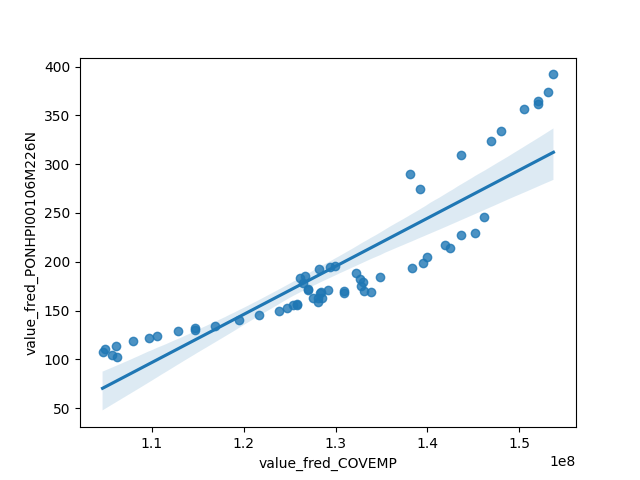
\includegraphics[scale = 0.9]{plots/plot_2026-10-29.png}
\caption{Raw Regression Plot for 2026-10-29}
\end{figure}
\newpage
\subsection{Detrended Regression}
\noindent Regresses the residuals of each series after removing its own linear time trend, so a shared trend can no longer drive the result on its own. A relationship that stays significant here is better evidence of a genuine link between the two series.

\begin{center}
\begin{tabular}{lclc}
\toprule
\textbf{Dep. Variable:}                 & value\_fred\_PONHPI00106M226N\_detrended & \textbf{  R-squared:         } &     0.170   \\
\textbf{Model:}                         &                   OLS                    & \textbf{  Adj. R-squared:    } &     0.156   \\
\textbf{Method:}                        &              Least Squares               & \textbf{  F-statistic:       } &     12.07   \\
\textbf{Date:}                          &             Thu, 29 Oct 2026             & \textbf{  Prob (F-statistic):} &  0.000965   \\
\textbf{Time:}                          &                 17:40:13                 & \textbf{  Log-Likelihood:    } &   -299.68   \\
\textbf{No. Observations:}              &                      61                  & \textbf{  AIC:               } &     603.4   \\
\textbf{Df Residuals:}                  &                      59                  & \textbf{  BIC:               } &     607.6   \\
\textbf{Df Model:}                      &                       1                  & \textbf{                     } &             \\
\textbf{Covariance Type:}               &                nonrobust                 & \textbf{                     } &             \\
\bottomrule
\end{tabular}
\begin{tabular}{lcccccc}
                                        & \textbf{coef} & \textbf{std err} & \textbf{t} & \textbf{P$> |$t$|$} & \textbf{[0.025} & \textbf{0.975]}  \\
\midrule
\textbf{const}                          &    4.801e-12  &        4.285     &  1.12e-12  &         1.000        &       -8.574    &        8.574     \\
\textbf{value\_fred\_COVEMP\_detrended} &    3.658e-06  &     1.05e-06     &     3.475  &         0.001        &     1.55e-06    &     5.76e-06     \\
\bottomrule
\end{tabular}
\begin{tabular}{lclc}
\textbf{Omnibus:}       &  4.556 & \textbf{  Durbin-Watson:     } &    0.081  \\
\textbf{Prob(Omnibus):} &  0.103 & \textbf{  Jarque-Bera (JB):  } &    3.381  \\
\textbf{Skew:}          &  0.437 & \textbf{  Prob(JB):          } &    0.184  \\
\textbf{Kurtosis:}      &  2.248 & \textbf{  Cond. No.          } & 4.07e+06  \\
\bottomrule
\end{tabular}
%\caption{OLS Regression Results}
\end{center}

Notes: \newline
 [1] Standard Errors assume that the covariance matrix of the errors is correctly specified. \newline
 [2] The condition number is large, 4.07e+06. This might indicate that there are \newline
 strong multicollinearity or other numerical problems.

\begin{figure}
\centering
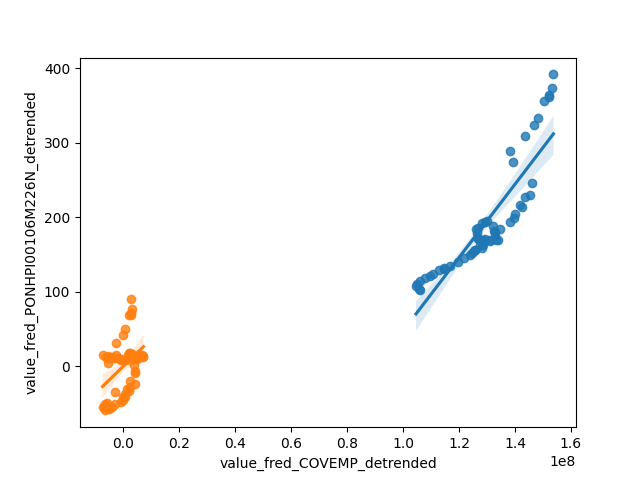
\includegraphics[scale = 0.9]{plots/plot_2026-10-29_detrended.png}
\caption{Detrended Regression Plot for 2026-10-29}
\end{figure}
\newpage
